%imports
%=============================================================================================
\documentclass[a4paper,12pt]{article}
\usepackage[spanish, english]{babel}
\usepackage[utf8]{inputenc}
\usepackage{booktabs}
\usepackage{listings}
\usepackage{fontawesome}
\usepackage{graphicx}
\graphicspath{ {Graficos/} }
\usepackage{gensymb}
\usepackage{natbib}
\usepackage{caption}
\usepackage{pdfpages}
\usepackage[export]{adjustbox}
\usepackage{subfig}
\usepackage{a4wide}
\usepackage[colorlinks=true,linkcolor=black,urlcolor=blue,bookmarksopen=true]{hyperref}
%\usepackage{bookmark}
\usepackage{fancyhdr}
\usepackage[spanish]{babel}
\usepackage[utf8]{inputenc}
\usepackage[T1]{fontenc}
\usepackage{graphicx}
\usepackage{float}
\usepackage{fancyvrb}
\renewcommand*\ttdefault{txtt}
\usepackage[T1]{fontenc}
\usepackage{listings}
\usepackage{amssymb}
\usepackage{setspace}
\usepackage{helvet}
\usepackage{lmodern}
\usepackage{titlesec}

%para el titulo de la tabla de contenidos
%=============================================================================================
\addto\captionsenglish{
  \renewcommand{\contentsname}
    {Indice}
}
%=============================================================================================



%comienzo de documento
%=============================================================================================
\begin{document}
\title{
    \includegraphics[width=10cm]{"Logo FIUBA".jpg}\newline
    Teoría de Algoritmos I 75.29\\
    Trabajo Práctico N\textsuperscript{\underline{o}} 1\
}
\author{Grupo Rosita Forever}
\date{}
\setlength{\parindent}{0pt}

\pagenumbering{gobble}
\maketitle

\begin{table}[h!]
    \centering
	\begin{tabular}{ccc}
	    \toprule
		Apellido y Nombre & Padrón & Correo electrónico	\\
		\midrule
		Jamilis, Netanel David   & 99093 & njamilis@fi.uba.ar\\
		Del Torto, Agustín       & 98867 & adeltorto@fi.uba.ar\\
		Daverede, Agustín        & 98540 & agusdaverede@yahoo.com.ar \\
		Betz, Joaquín            & 104348 & \\
		\bottomrule
	  \end{tabular}
\end{table}
	
\verb Github: \faGithub \quad \faGithubSign \par
\extrainfo{
\url{{https://github.com/netaneldj/7529-TDA/TP1}} \newline}
\newpage
\pagenumbering{arabic}
\tableofcontents
\newpage

%secciones
%=============================================================================================
\section{Introducción}

\subsection{Objetivos}
Los objetivos del presente trabajo son los siguientes:
\begin{itemize}
\item Aplicar los conceptos aprendidos en clase en un problema Greedy
\item Aplicar los conceptos aprendidos en clase en un problema de División y Conquista
\item Preparar un informe técnico
\end{itemize}

En las siguientes secciones se vera plasmado el cumplimiento de los objetivos.\newline

\subsection{Resumen}
El presente trabajo se centrará en la presentación y consecuente resolución de los problemas planteados.\newline 
En primer lugar, se tratará el problema de ausentismo, perteneciente a la familia de problemas Greedy. Se analizará su solución y se planteará explicando el algoritmo empleado paso a paso.
Luego, se repetirá el mismo análisis para el problema de una nueva regulación industrial, donde se aplicará la estrategia de división y conquista.

En último lugar, se analizaran los resultados obtenidos, donde se tendrán en cuenta los conocimientos adquiridos en el desarrollo del trabajo y la bibliografía consultada para la realización del presente informe.

\newpage

 \section{Manifestaciones seguras}

En una decisión temeraria una ciudad decidió autorizar un conjunto de n manifestaciones el mismo día y horas. Cada manifestación comienza en un punto de reunión y tiene un destino final. Para evitar enfrentamientos y confusiones desean que cada ruta sea aislada de las otras. Contamos con el mapa de la ciudad que incluye todos los caminos e intersecciones por lo que pueden ir las marchas. Nos piden que elaboremos un algoritmo que retorne los caminos a seguir para cada manifestación de modo que no haya riesgo de un cruce (si es posible).\newline
Debemos demostrar que es un problema NP-Completo.
%=============================================

\subsection{Solución}
El problema que precede se puede modelar con un grafo en donde los nodos son las intersecciones de las calles y las aristas son las calles de la ciudad. En un principio todas las calles están disponibles para efectuar las manifestaciones siempre y cuando no se superpongan las manifestaciones.
%=============================================

\subsection{Demostración NP-Completo}
Para demostrar que es $\mathsf{NP-Completo}$ debemos demostrar que nuestro problema pertenece a $\mathsf{NP}$ y a $\mathsf{NP-Hard}$ simultáneamente.

\subsubsection{Demostración NP}
Para demostrar que el problema es $\mathsf{NP}$ debemos poder corroborar la solución propuesta en tiempo polinomial. Usando la analogía de la cerradura y la llave, esto sería equivalente a dada la llave probar que esta abre la cerradura en "tiempo polinomial". \newline

A continuación se propone un algoritmo que verifica la solución propuesta en tiempo polinomial:

\begin{verbatim}
Llamar L a la lista de manifestaciones(representadas por tuplas de nodos)

Funcion esManifestacionValida(L):
    Llamar visitados a la lista que contendrá a los nodos visitados
    
    visitados es lista vacia
    Para cada manifestacion en manifestaciones:
        Para cada esquina en manifestacion:
            Si esquina en visitados:
                Devolver falso
            Sino:
                visitados agregar esquina
    Devolver verdadero
\end{verbatim}

Se puede apreciar que la complejidad es de $\mathcal{O}(km)$ siendo $k$ la cantidad de manifestaciones y $m$ la cantidad máxima de esquinas atravesadas por una manifestación.

\subsubsection{Demostración NP-Hard}
Para demostrar que el problema es $\mathsf{NP-Hard}$, consideremos una instancia del problema conocido como conjunto independiente que consiste en un grafo $G=(V, E)$ con $|V|=n$ y un valor entero $k$.

\begin{figure}[H]
\centering
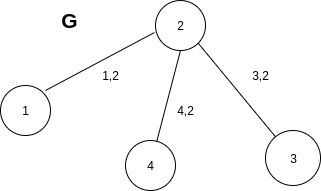
\includegraphics[width=0.9\textwidth]{Informe/Imagenes/Parte1/grafico 1.png}
\caption{\label{fig:class01}Instancia conjunto independiente}
\end{figure}

Sea el grafo $M = (V', E')$ donde $V' = V \cup \{ x_{u,v} \, : \, (u,v) \in E \}$ y $E' = V' \times (V'-1)$.

\begin{figure}[H]
\centering
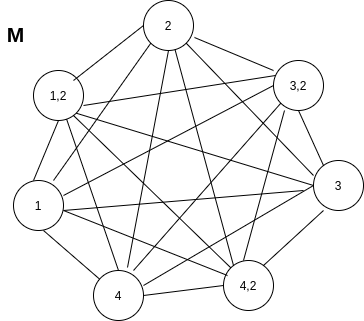
\includegraphics[width=0.9\textwidth]{Informe/Imagenes/Parte1/grafico 2.png}
\caption{\label{fig:class01}Grafo manifestaciones}
\end{figure}

Para cada $u \in V$ siendo $v_1, v_2, \dots, v_m$ los vecinos de $u$ en $G$ y definamos la ruta $P_u = \langle u, x_{u,v_1}, x_{u,v_2}, \dots, x_{u,v_m} \rangle⟩$ en $M$. Siendo $\mathcal{P} = \{P_u \, : \, u \in V\}$.\newline

Hay un conjunto independiente de tamaño como máximo $k$ en $G$, si y solo si hay un subconjunto $\mathcal{P}'$ con $|\mathcal{P}'| \le k$ tal que los caminos en $\mathcal{P}'$ son vértices disjuntos. \newline
Para visualizarlo, construimos los siguientes Paths en M: 

\begin{figure}[H]
\centering
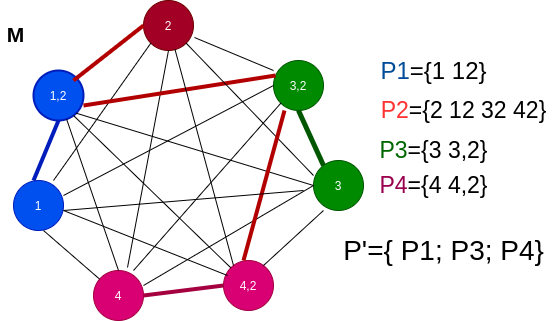
\includegraphics[width=0.9\textwidth]{Informe/Imagenes/Parte1/grafico 3.png}
\caption{\label{fig:class01}Rutas}
\end{figure}

Ahora queda formado un $\mathcal{P}'$ =  \{ P1; P3; P4 \} con $|\mathcal{P}'| = 3$ que representa en nuestro grafo G:

\begin{figure}[H]
\centering
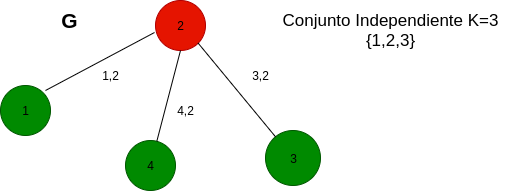
\includegraphics[width=0.9\textwidth]{Informe/Imagenes/Parte1/grafico 4.png}
\caption{\label{fig:class01}Nodos Independientes}
\end{figure}

Más precisamente, si $S$ es un conjunto independiente de $G$, entonces $\{ P_u \, : \, u \in S \}$ es una colección de caminos separados de vértices $M$ y, si $\mathcal{P}'$ es una colección de caminos separados de vértices en $M$, entonces $\{u \, : \, P_u \in \mathcal{P}' \}$ es un conjunto independiente de $G$.

\begin{figure}[H]
\centering
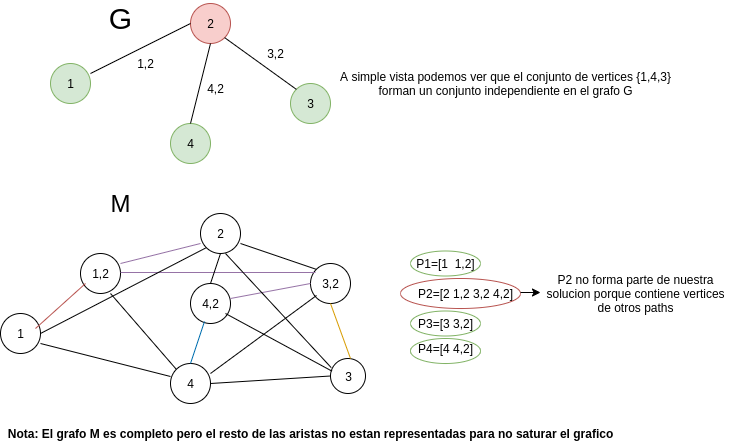
\includegraphics[width=1.148\textwidth]{Informe/Imagenes/Parte1/grafico 5.png}
\caption{\label{fig:class01} Vista General}
\end{figure}
%=============================================



\newpage

\section{División de Bienes}

Una de las parejas más ricas del mundo está pasando por un proceso de divorcio. Entre sus bienes cuentan con propiedades, autos, motos, estampillas raras y otros coleccionables. Como no se ponen de acuerdo en la manera de dividirlos, el juez ha dictaminado que un tasador ponga valor a cada bien y luego se haga una partición por valores iguales. El juez nos pide que elaboremos un algoritmo que en forma eficiente haga este trabajo.<<\newline
%============================================

\subsection{Solución}
El problema que precede se puede pensar como una representación de un conjunto

$C=\{w_{1}, w_{2}, ..., w_{n}\}$ donde cada $w_{i}$ está asociado al precio de cada bien. Luego, se desea determinar si existe un subconjunto de C tal que:

\begin{equation}
    W=\sum w_{i}
\end{equation}

Donde $w_{i}$ representa el precio de cada bien.

Utilizando conceptos de programación dinámica es posible llegar a una solución. No obstante, dicha solución estaría caracterizada por ser $O(W\cdot n)$, donde n es la cantidad de bienes y W es el valor de la ecuación (1) al que se desea llegar. Esto puede llegar a ser de orden casi exponencial si considera un W muy grande, y se tiene en cuenta la cantidad de bits empleados para representarlo y su crecimiento.

Sin embargo, como se describirá en el siguiente apartado, el problema es NP-Completo, de manera que no es posible hallar una solución que no sea exponencial. Al menos así ha sido descripto hasta ahora.

\subsection{Demostración NP-C}
%=============================================
Para poder demostrar que el problema es NP-Completo, se decidió proceder realizando la demostración a partir de dos hipótesis:
\begin{itemize}
    \item El problema es NP
    \item El problema es NP-Hard
\end{itemize}

Si ambas se cumplen, podemos afirmar que el problema es NP-Completo.

En primer lugar, se debe demostrar que es NP. Utilizando la notación previa, se puede decir que el subconjunto C puede tener tantos elementos como el conjunto original. Para poder hallar a W es preciso realizar las sumas asociadas a las iteraciones de los diferentes $w_{i}$. Esto se puede resolver en tiempo polinomial, luego el problema es NP.

Ahora se debe probar que el problema es NP-Hard. 

Para eso se va a demostrar:

\begin{equation}
    3DM \leq_{p} SUBSET-SUM
\end{equation}

La demostración se sustenta en que es conocido que el problema 3 dimensional matching es NP-C.

Para proceder a demostrar que el problema SUBSET SUM se puede reducir a 3DM se planteará que el conjunto C\subseteq X,Y,Z, siendo estos conjuntos ordenados disjuntos de tamaño n cada uno. Se desea determinar si existe el conjunto C.

Luego, se procede a representar a una tripla $t={x_{i}, y_{i}, z_{i}}$ como una serie de bits de tamaño 3n. A los efectos de resolver el problema se plantea que el conjunto C se puede representar como se demuestra a continuación:

\begin{figure}[H]
\centering
\includegraphics[width=0.7\textwidth]{Informe/Imagenes/Parte2/imagen1.png}
\caption{\label{fig:class01}Representación de tripla}
\end{figure}

No obstante, esta representación trae aparejado un posible problema de overflow. Esto se puede observar en la siguiente representación:

\begin{figure}[H]
\centering
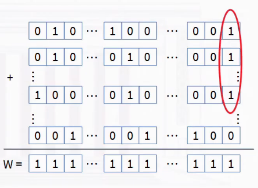
\includegraphics[width=0.5\textwidth]{Informe/Imagenes/Parte2/imagen2.png}
\caption{\label{fig:class01}Problema de overflow}
\end{figure}

Para evitar esta situación se debe elegir una representación en una base al menos un valor mayor de la cantidad de triplas, ya que esto imposibilita que se presente el overflow.

Al llegar a una representación del problema que se puede caracterizar por 3DM, podemos afirmar que el mismo representa a un problema similar a 3DM. 

Por lo tanto, como 3DM es NP-C, se probó la ecuación (2) y también que el problema es NP, se puede afirmar que se trata de un problema NP-C.
\newpage

\section{Conclusión}
Habiendo culminado el trabajo podemos efectuar las siguientes conclusiones:
%=============================================
 \subsection{Manifestaciones seguras}    
\begin{itemize}
    \item El problema se simplifica al modelar la ciudad como un grafo.
    \item Cada vértice independiente en \emph{Independet set} equivale a un camino independiente en nuestro problema
\end{itemize}
%=============================================
 \subsection{División de Bienes}    
\begin{itemize}
    \item 
\end{itemize}
%=============================================
\subsection{Un poco de teoría}    
\begin{itemize}
    \item Un problema solo puede ser resuelto por otro igual o más complejo que el primero
\end{itemize}
%=============================================

\newpage

\section{Bibliografia y Referencias}
\begin{itemize}
    \item J. Kleinberg, E. Tardos, Algorithm Design
    \item T. Cormen, C. Leiserson, R. Rivest, C. Stein, Introduction to Algorithms
    \item  Dr. Andrew Harrington, "Comp 363: Algorithms - Spring 2019" - Universidad Loyola Chicago.
\end{itemize}
 %=============================================
\newpage

\end{document}
%=============================================================================================
